\chapter{Explicit Generative Models}
\section{Variational Autoencoder}

Our goal is to find the data distribution $p(X)$. \Cref{fig:dgm} represents a general structure of deep generative model. As you can see, we first sample $z\sim p(z)$ and feed it into a deep neural network $f(z)$ and output $x$.

\begin{figure}[h]
	\begin{center}
		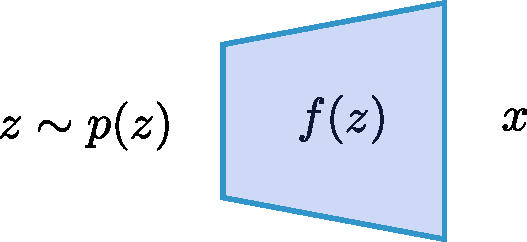
\includegraphics[scale=0.5]{./images/generative/dgm.pdf}
	\end{center}
	\caption{General structure of deep generative models. This model does not infer $z$ from $x$.}
	\label{fig:dgm}
\end{figure}

VAE performs an inference by introducing a probabilistic encoder, called inference network. VAEs are generative model with a latent variable distributed according to some distribution $p(z_i)$. The observed variable is distributed according to a conditional distribution 
$$p_\theta(x_i|z_i)$$
This conditioning means the latent variable values are the one most likely given the observations. We also create a distribution $q_\phi(z_i|x_i)$. We would like to be able to encode our data into the latent variable space. Let's model the distribution.

\begin{itemize}
	\item $p_\theta(x_i|z_i)\sim \mathcal{N}(x_{i}|\mu(z_i), \sigma^2(z_i))$: A probabilistic decoder (or generative network, $\theta$)
	\item $q_\phi(z_i|x_i)$: A probabilistic encoder (or inference network $\phi$). We can choose a family of distributions for our conditional distribution $q$ (\eg standard Gaussian distribution). 
		$$q_\phi(z_i|x_i) = \mathcal{N}(z_i|\mu(x_i, W_1), \sigma^2(x_i, W_2)I),$$
	where $W_1$ and $W_2$ are network weights and collectively denoted as $\phi$. We create a neural network to model the distribution $q$ from our data in a non-linear manner. The outputs of the network are $\mu$ and $\sigma$. 
\end{itemize}

\begin{figure}[h]
	\begin{center}
		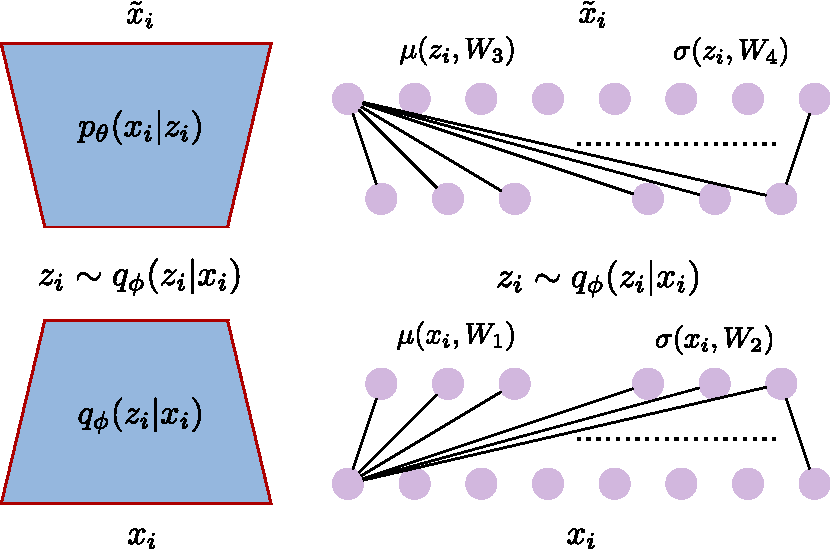
\includegraphics[scale=0.5]{./images/generative/encoder.pdf}
	\end{center}
	\caption{Overview of variational autoencoder.}
	\label{fig:vae}
\end{figure}



\begin{align*}
	p(X,Z|\theta) &=  \prod_{i=1}^{n}\underbrace{p(x_i|z_i,\theta)}_{\textrm{Likelihood, Generator}}\underbrace{p(z_i|\theta)}_{\textrm{Prior on latent variable}}\\
	&= \prod_{i=1}^{n} \mathcal{N}(x_{i}|\underbrace{\mu(z_i), \sigma^2(z_i)}_{\textrm{Non-linear}}) \mathcal{N}(z_i|0, I)
\end{align*}

Subsequently, marginal distributions can be expressed as follows under i.i.d. assumption:
\begin{align*}
	p(X|\theta) &= \prod_{i=1}^{n} p(x_i|\theta) \\
	&= \prod_{i=1}^{n} \int p(x_i, z_j|\theta) dz_j \\
	& = \prod_{i=1}^{n} \int p(x_i|z_i, \theta)p(z_i|\theta)dz_i \\
	& = \prod_{i=1}^{n} \int \mathcal{N}(x_{i}|\mu(z_i), \sigma^2(z_i)) \underbrace{\mathcal{N}(z_i|0, I)}_{\textrm{Mixture weight}} dz_i
\end{align*}

\begin{itemize}
	\item As you can see, the marginal distribution $p(X|\theta)$ becomes a mixture of Gaussian (infinite mixture of Gaussian). 
	\item Even though $p(x|z)$ and $p(z)$ are normal, $p(x)$ is not normal, because it is a mixture distribution.
	\item The non-linearity of Gaussian parameters (modeled by a neural network), conjugacy between the prior and the likelihood does not hold anymore.
%	\item Diagonal covariance matrix does not mean the independence between elements of $x$.
	\item Again, $\mu$ and $\sigma$ is non-linear function of $z$ modeled by some non-linear neural network. The neural network works as a powerful non-linear parameter approximator (based on universal approximation theorem). 
	\item Simple prior is used. Let's consider the data $x$ is an image of $100\times 100$ pixels. Then the covariance matrix has to be $10000\times 10000$. Thus, it is common to set a simple prior such as the standard Gaussian (covariance matrix is diagonal matrix). However, even if we set a simple distribution, with the infinite mixture of Gaussian, we can model any distribution.
	\item VAE uses a global parametric model to predict the local
		variational parameters for each data point (\textbf{amortized inference}). 
%	\item Under the simple standard Gaussian prior assumption, the generator, $p(x_i|z_i,\theta)$, returns factorized Gaussian whose mean and variance are non-linear functions of latent variable modelled by deep neural network parameterized by $\theta$.
%	$$p(x_i|z_i,\theta) = \mathcal{N}(x_{i}|\mu(z_i), \sigma^2(z_i))$$
%	\item VAEs uses a simple prior over latent variables and complicated and powerful generator (neural network).
	\item It allows to convert complicated large-dimensional data distributions into simple lower-dimensional latent variable representations.  
%	\item $Std = e^{\frac{1}{2}\log (Var)}$, thus output is the log var
\end{itemize}

\subsection{VAE Optimization}
We can train VAE using variational inference with the following objective function, ELBO:
$$\mathcal{L}(\phi,\theta) = \mathbbm{E}_{q_{\phi}(z|x)}[\log p_{\theta}(x|z)] - D_{\textrm{KL}}(q_{\phi}(z|x)||p_{\theta}(z))$$
Let's closely look at this objective function:
\begin{itemize}
	\item In $q_{\phi}(z|x)$, $x$ is a given data, so it is not stochatic. How to sample $z$?
	\item $q$ has to be deterministic and differentiable. 
	\item[] $\to$ \textbf{Reparameterization trick}!
		$$\tilde{z}\sim q_\phi(z|x) \to \tilde{z}\sim g_{\phi}(\epsilon, x)$$, where $\epsilon\sim p(\epsilon).$

	\item Estimated by using Monte-Carlo estimation 
		$$\mathbbm{E}_{q_{\phi}(z|x)}[\log p_{\theta}(x|z)]\approx \frac{1}{N}\sum_j \log p_{\theta}(x_i|z_j).$$
\end{itemize}

\subsection{Conditional VAE}
If we have label information about data, then it would provide a better optimization of VAE model. Recall that the following objective function is the objective of the original VAE:
$$\mathcal{L}(\phi,\theta) = \mathbbm{E}_{q_{\phi}(z|x)}[\log p_{\theta}(x|z)] - D_{\textrm{KL}}(q_{\phi}(z|x)||p_{\theta}(z))$$
In conditional VAE, 
$$\mathcal{L}(\phi,\theta) = \mathbbm{E}_{q_{\phi}(z|x, y)}[\log p_{\theta}(x|y, z)] - D_{\textrm{KL}}(q_{\phi}(z|x, y)\ ||\ p_{\theta}(z|y))$$

\begin{align}
	\log p(X|Y) & = \ln\int q(Z|X, Y) \frac{p(X, Z|Y)}{q(Z|X, Y)}dZ\\
					 & \geq \underbrace{\int q(Z|X, Y) \ln\frac{p(X, Z|Y)}{q(Z|X, Y)}dZ}_{\textrm{ELBO, } \mathcal{L}(q,\theta)} \quad\textrm{by Jensen's Inequality.}\\
					 &\dots\\
					 &\dots\\
					 &= \mathbb{E}_{q(Z|X,Y)} [\ln p(X|Z,Y)]  - KL(q(Z|X,Y)||p(Z|Y)) 
	% & = \int q(Z)\log \frac{p(X,Z|\theta)}{p(Z|X,\theta)}dZ\\
	% & = \int q(Z)\log \frac{q(Z)p(X,Z|\theta)}{q(Z)p(Z|X,\theta)}dZ\\
	% & = \int q(Z)\log \frac{p(X,Z|\theta)}{q(Z)}dZ+ \int q(Z)\log \frac{q(Z)}{p(Z|X,\theta)}dZ\\
	% & = \underbrace{\int q(Z)\log \frac{p(X,Z|\theta)}{q(Z)}dZ}_{\textrm{ELBO, } \mathcal{L}(q,\theta)}+ \textrm{KL}(q(Z)||\log p(Z|X,\theta))
\end{align}
Note that not we have a prior $p_{\theta}(z|y)$. However, we have no idea about latent variable $z$, so we simply assume that we cannot impact the $z$ by $y$. Thus, we typically set it as a standard normal distribution. Also, we can simply concatenate the input $X$ with $Y$. 

\subsection{Variational Deep Embedding (VaDE)}
The generative process of VADE $p(x, z, c) = p(x|z)p(z|c)p(c)$:
\begin{itemize}
	\item Choose a cluster $c\sim Cat(\pi)$
	\item Choose a latent vector $z\sim \mathcal{N}(\mu_c, \sigma_c^2I)$
	\item Choose a sample $x$:
		\begin{align*}
			x\sim
			\begin{cases}
				Ber(\mu_x)\quad &\textrm{If }$x$ \textrm{ is binary} \\
				\mathcal{N}(\mu_x, \sigma_x^2I) \quad &\textrm{else}
			\end{cases}
		\end{align*}
\end{itemize}
ELBO of VaDE:
\begin{align}
	\log p(X) & = \ln\int \sum_c p(X,Z,C) dz \\
					 & \geq \underbrace{\int q(Z,C|X) \ln\frac{p(X, Z, C)}{q(Z,C|X)}dZ}_{\textrm{ELBO}} 
\end{align}
The ELBO can be decomposed as follows:
\begin{align*}
\mathcal{L}_{ELBO} &= \mathbb{E}_q(z,c|x)\bigg[\ln\frac{p(x,z,c)}{q(z,c|x)}\bigg]\\
				   &= \mathbb{E}_q(z,c|x)[\ln p(x,z,c) - \ln q(z,c|x)]\\
				   &= \mathbb{E}_q(z,c|x)[\ln p(x|z) + \ln p(z|c)+ \ln p(c)-\ln q(z|x)-\ln q(c|x)]
\end{align*}
By using two factorizations:
\begin{itemize}
	\item $p(x, z, c) = p(x|z)p(z|c)p(c)$
	\item $q(z,c|x) \approx q(z|x)q(c|x)$ (Mean-field assumption)
		\begin{itemize}
			\item $q(z|x)\sim \mathcal{N}$: encoder, estimate mean and variance.
			\item $q(c|x)$: assignment probability of Gaussian mixture model
		\end{itemize}
\end{itemize}

\subsection{Importance Weighted VAE}


% \begin{itemize}
% 	\item 
% 		$$\mathbbm{E}_{q_{\phi}(z|x)}[\log p_{\theta}(x|z)]\approx \frac{1}{N}\sum_j \log p_{\theta}(x_i|z_j).$$
% 	\item The second term can be solve analytically for some distributions like Gaussian.
% 	\item For training, we need to use a reparameterization trick. 
% \end{itemize}




%\footnotetext[1]{Uncorrelated relationship does not imply the independence (independence makes covariance to be diagonal). If two variables are uncorrelated, $Cov(x_i,x_j)=0 $, there is no linear relationship between them.}
%\footnotetext[2]{In practice, simple prior could be a problem.}
